\chapter{Introduction}

Currently, pests and pathogens threaten the survival of numerous tree species around the globe. 
An upsurge in the trade and transport of non-native plants and the widespread adoption of monoculture plantations have drastically increased the risk of large-scale outbreaks in native tree populations.
Moreover, following the effects of climate change and increased temperatures, the threats posed by invasive non-indigenous pathogens are only set to increase. Accordingly, efforts to understand the precise mechanisms that underpin epidemics in tree populations are essential for human wellbeing and ecosystem stability.

When an epidemic takes hold, numerous challenges complicate an effective on-the-ground response. In addition, epidemic drivers are multifaceted, hard to quantify, and often unknown. 
Consequently, epidemic models are significantly challenging to parameterise. 
Further still, communicating research insight to policymakers and stakeholders poses a significant challenge for modellers even with accurate parameterisation.

Despite the complex challenges that threaten tree health, scientists, policymakers, and stakeholders can cooperate to prevent the spread of emergent infectious tree diseases within a country.
Notably, the output from mathematical models can help advise practical management strategies to control epidemics through rural and urban tree populations.
Accurate epidemic models can also help forest and woodland managers structure plantations to minimise epidemic impact. 
Aiding forest managers with mathematical models has become particularly vital given the UK government's recent measures to sequester carbon from the atmosphere with land-use change and afforestation, thereby increasing tree coverage throughout Great Britain.

This Chapter introduces the reasons, challenges, and value in modelling tree disease epidemics.
First, the overarching rationale behind researching tree disease models is highlighted, followed closely by reviewing the most pressing epidemic drivers.
Second, the challenge of implementing epidemic control is summarised, along with the principal socioeconomic relationships between modellers, policymakers and stakeholders. Finally, the Chapter concludes by outlining the topics covered in this thesis.


\section{Invasive tree diseases}

The modern world relies heavily on imports and exports characterised by global trade networks. 
Unfortunately, the trade and transport of foreign plant material can introduce invasive pests and pathogens into non-native landscapes. 
As such, crops, flowering plants and tree populations that lack evolutionary adaptations 
to these invasive (pathogenic) species face unprecedented perils \cite{doi:10.1002/9781444329988.ch8}.
Epidemics through botanical populations can be devastating.
Classic historical examples include Irish potato blight, Dutch elm disease (\acrshort{ded}) \cite{doi:10.1111/j.1365-3059.2010.02391.x} 
and North American chestnut blight \cite{doi:10.1002/9780470535486.ch7}.
Two high-profile epidemics currently underway in the UK include ash dieback (\acrshort{adb}) affecting European ash \textit{Fraxinus excelsior} (\acrshort{fe})
\cite{ash-dieback-costs}, and \textit{Phytophthora ramorum} (\acrshort{pr}), a prevalent disease affecting over 150 plant species, including oak, 
larch, and sweet chestnut \cite{p.ramourum}.

Given the fundamental significance of tree populations in terrestrial ecosystems, ensuring tree health forms a critical challenge for society to address.
In particular, policymakers can lead control initiatives to help impede the spread of disease \cite{Gilligan-disease-management}.
However, implementing an uninformed and ineffective management strategy is costly and does little to stop the spread.
Accordingly, research into optimal disease management underpins the central issue of botanical epidemiology, 
where research should ideally seek to minimise both epidemic and economic impact \cite{ash-dieback-costs, freer2017tree, boyd2013consequence, tyrvainen2005benefits}. 
Frequently, control strategies include reducing tree densities \cite{pietzsch2021effect, resiliency-density-reductions} and planting genetically diverse host distributions \cite{doi:10.1094/PD-89-0969, genetic-heterogeneity, huang1980importance}.

\subsection{Epidemic drivers}

The terms `pest' and `pathogen' describe a broad spectrum of taxonomically diverse organisms. Pests denote any organism that harms humans or human interests, such as crops or livestock \cite{buckle2015rodent, oerke2006crop, de1964biological}. Overwhelmingly, insects constitute the main
pest threats to tree species \cite{metcalf1994introduction}. In Great Britain (\acrshort{gb}), the Asian longhorn beetle (\acrshort{alb}) \cite{haack2010managing}, and oak processionary moth (\acrshort{opm}) \cite{tomlinson2015managing} are two such pests that currently threaten tree health.
In contrast, the term `pathogen' describes any organism that induces disease. In the context of tree populations, diseases include fungi, bacteria, viruses, and oomycetes \cite{balloux2017q, Boyd1235773}. Presently, the oomycete \textit{P. ramorum} \cite{brasier2005phytophthora}, and ADB
caused by the fungus \textit{H. fraxineus} (\acrshort{hf}) \cite{ash-dieback-costs, mitchell2014ash} are two pathogens that threaten tree-health in GB.

Tree pathogens have evolved diverse reproductive modes and epidemiologies,  characterising a distinctive challenge when controlling tree-based pathogens. Two contrasting examples include chestnut blight caused by the bark pathogen fungus \textit{ Cryphonectria parasitica} and the xylem inhibiting bacterium \textit{Xylella fastidiosa}\footnote{Several diseases are symptomatic expressions of \textit{X. fastidiosa}, including phoney peach disease, quick olive decline, coffee leaf scorch, and most notably, Pierce's disease affecting Grapes and citrus variegated chlorosis \cite{hopkins2002xylella}.}. 
Chestnut blight devastated American chestnut populations in the 1930s \cite{doi:10.1002/9780470535486.ch7}, and more recently, infections have been spreading through European chestnuts, albeit to a lesser extent \cite{heiniger1994biological}.
The principal infection mechanism of \textit{ C. parasitica} occurs through windborne spore dispersal into wounds or openings in bark. 
In contrast, transmission of the bacterium \textit{X. fastidiosa} is thought to occur exclusively through sap-sucking insect vectors, e.g leafhoppers of the genus \textit{Homoptera} \cite{redak2004biology}. 
One remarkable facet of \textit{X. fastidiosa} is its ability to infect numerous tree species. Current estimates indicate the host range of \textit{X. fastidiosa} is upwards of 611 different plant species \cite{european2022update}, whereas \textit{C. parasitica} predominantly infects chestnut species and occasionally nearby oak \cite{rigling2018cryphonectria}. 

The trade and transport of non-native plant material are widely recognised to risk introducing invasive pests and pathogens into native landscapes \cite{POTTER201761, lovett2016nonnative, roy2014increasing}.
Ensuing epidemics can overwhelm botanical species lacking genetic resistance to the invasive species \cite{desprez2016evolutionary}, better understood from an evolutionary perspective: in a natural environment unaltered by human transportation, tree species co-evolve with invasive pathogens in a `gene-for-gene' arms race \cite{Thrall1735, dangl2001plant, flor1971current}.
The spread of Dutch elm disease in the UK \cite{doi:10.1111/j.1365-3059.2010.02391.x} and chestnut blight
in North America \cite{doi:10.1002/9780470535486.ch7} are two classic examples that shook the world.

Trade regulations on plant imports are essential to prevent the initial introduction of invasive pathogens \cite{rodoni2009role}, exemplified by the Dutch elm disease epidemic in the UK. 
Had more stringent regulations been active in the 1960s, elm timber infected with scolytid bark beetles (carrying the fungus \textit{Ophiostoma novo‐ulmi}) might have prevented the devastating outbreak \cite{doi:10.1111/j.1365-3059.2010.02391.x}. 
Ordinarily, these preventative measures take the form of customs checks on imported/exported timber, crops or horticultural goods. 
Recently, the European Commission enacted plant passports to regulate how growers and traders can transport plant material between countries \cite{wulfert2010implementation}.

If checks and policy implementations fail, a pathogen might be introduced into the landscape and spread through natural
dispersal pathways. Alternatively, a pathogen might be transported into foreign ecosystems through atmospheric 
long distance dispersal (\acrshort{ldd}) \cite{brown2002aerial}. In any case, biological control becomes necessary. 
The biological control of plant-based disease
can be achieved in numerous ways. Commonly, this involves chemical agents such as pesticides, predatory insects or planting
genetically resistant cultivars \cite{pal2006biological, baker1974biological}. 

In this work, we aim to construct epidemic models and investigate eradication strategies
entailing the removal of trees through sanitation felling. 
In this pursuit, three questions are vital to consider: 
(1) How do we effectively identify an infected tree? 
(2) How can we optimise tree felling to slow the spread of disease given limited resources/budgets?
(3) What is the risk that a large-scale epidemic will result from the initial observations of diseased trees?

\section{Modelling and policy}
\label{sec:modelling-and-policy}

The benefit of controlling an epidemic should outweigh the costs of letting an outbreak spread unchecked. 
Plant disease modellers can help infer well-designed control policies that maximally reduce epidemic impact and minimise the expenditure
of resources\textemdash both natural and economic. However, achieving this in practice is problematic due to various unknowns \cite{13-challenges}, and history gives examples of insufficient control policies that fail to halt pathogen spread. 
Prominent examples include the mismanagement of Dutch elm disease in the late 1960s and early 1970s \cite{dutch-elm-mismanage}, and more recently citrus canker in Florida \cite{schubert2001meeting}.

We can attempt to understand what dictates the optimal control of tree disease epidemics with mathematical models. 
Control strategies have been explored on both smaller \cite{risk-potential-control} and larger landscapes \cite{large-scale-control2}. 
On all spatial scales, consensus agrees that the effort and resources required to control an epidemic depend significantly on the scale of the epidemic at hand. That is, \textit{'aggressive pathogens should be met with aggressive control'}, as confirmed by modelling studies \cite{control-scale-matching, WEBIDEMICS}. 
In any scenario, an on-the-ground response must be carried out swiftly. Otherwise, the likelihood of successful management decreases rapidly, and the cost of inaction soars.
% 1. Examples of where modelling work has been used to inform control...

Conventional eradication strategies involve detecting symptomatic trees and culling neighbours within a radius, e.g. \cite{WEBIDEMICS}.
A naive strategy that indiscriminately culls hosts can be fine-tuned and optimised to maximally reduce the epidemic impact. 
For example, one strategy prioritises targets by ranking hosts according to expected number of secondary infections \cite{risk-potential-control}.
Over larger spatial scales, models of sudden oak death (\acrshort{sod}) in California indicate that epidemics are most effectively controlled by targeting infected trees either at or ahead of the infectious wave-front \cite{large-scale-control}.
Nevertheless, various factors complicate eradication regardless of the spatial scale, such as the cryptic nature of tree diseases and fluctuating government budgets \cite{control-theory, control-theory-application}.

Enhanced surveillance and monitoring strategies also seek to optimise resource allocations. 
Surveillance aims to detect infected individuals and disease incidence, generally requiring the collection and analysis of epidemic data \cite{surveillance-review}.
Ultimately, surveillance and monitoring comprise the last line of defence after preemptive border checks and inspections have failed to prevent the introduction of disease. 
Statistical approaches have been adopted to optimise the number of samples/surveys required to infer disease incidence accurately \cite{yamamura2016sampling}.
Moreover, optimal surveillance strategies have been examined with logistic \cite{parnell2012estimating} and mechanistic \cite{WEBIDEMICS} epidemic models\textemdash the next Chapter offers a more in-depth review of these modelling paradigms. 

Several governmental bodies have a stake in the surveillance and monitoring of tree health in the UK, often collaborating their efforts. For example, the National Forest Inventory (NFI) conduct general surveys to determine tree distributions and woodland composition\textemdash discussed more in section \ref{ch2:hostdata}. Subsequently, output from NFI surveys is utilised by  'Forestry Research' (FR), the research agency of the Forestry Commission (FC). In addition, the FC plays a vital role in surveying landscapes for infectious tree diseases in the UK \cite{ryle1969forest, james1990history}, often responding to high-risk invasions in a more targeted capacity. Historically, the UK government has tasked the FC to undertake comprehensive large-scale surveys in response to Dutch elm disease in the 1960s-1970s \cite{potter2011learning} and ash dieback in 2012 \cite{tomlinson2016discovery}. 
However, citizen science-based approaches have become increasingly utilised to monitor tree health \cite{brown2020role}, exemplified by the monitoring tool 'TreeAlert', a website owned by FR designed to collect information about tree health in woodlands and forests through user reports.

Even supposing an accurate and well-informed control strategy,
a response on the ground only ensues when stakeholders implement control initiatives \cite{reed2018theory}. Here, the term `stakeholder' is extensive, reflecting any interested individual, collective, or organisation with a stake in tree health that has the potential to influence or affect a policy direction or control decision \cite{brugha2000stakeholder}. The UK's stakeholder landscape for tree health is equally broad, encompassing diverse governmental and private sector organisations and individuals. A conceptual framework for stakeholder categorisation was put forward by \cite{dandy2017has}, alongside a case study of who had a stake in ash dieback in the UK. In their analysis, \cite{dandy2017has} listed various affected stakeholders:
\begin{itemize}
    \item \textbf{governmental}: DEFRA, FERA, FC, FR and various local authorities
    \item \textbf{civil society/third sector}: National Trust, Wildlife Trust, Woodland Trust
    \item \textbf{private sector}: private land managers, outdoor recreationists, forest owners, citizen scientists, and the general public
\end{itemize}

\begin{figure}
    \centering
    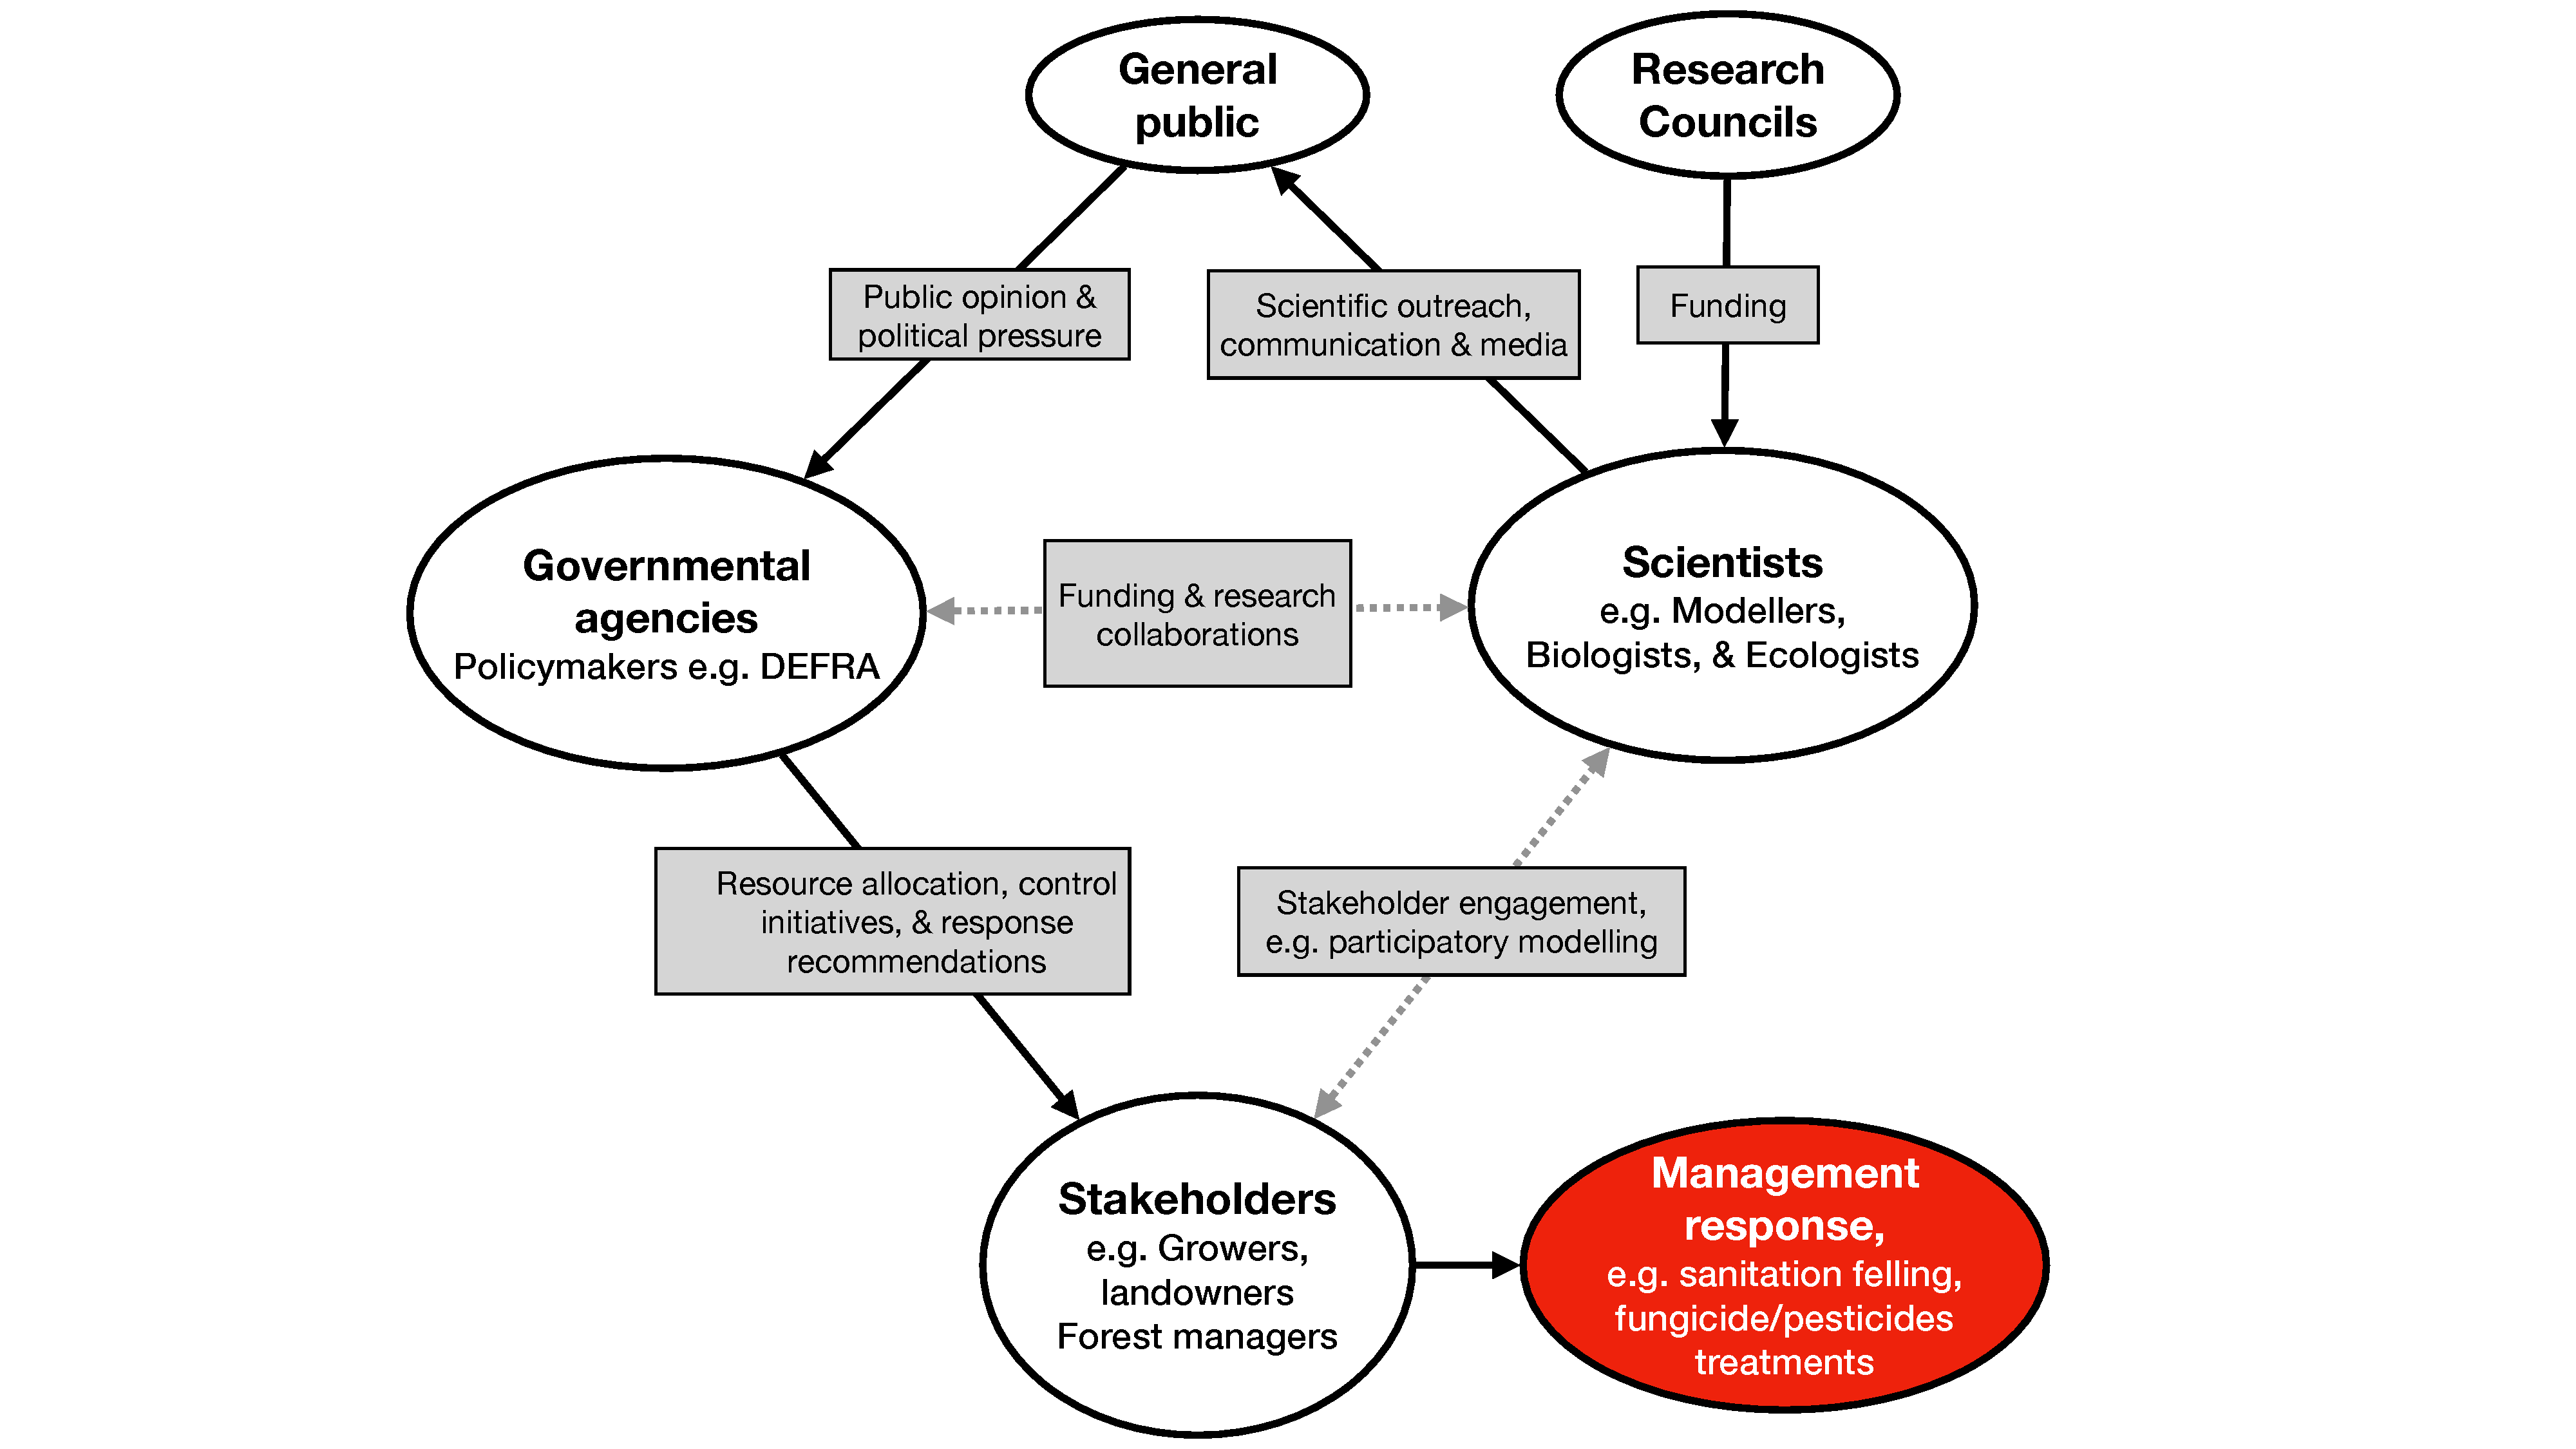
\includegraphics[scale=0.35]{chapter1/figures/modelling-and-policy.pdf}
    \caption{A simplified model representing the major socioeconomic interactions between the general public, scientists, 
    policymakers and stakeholders in the UK. Scientists receive funding from and collaborate with Governmental bodies/policymakers. 
    Policymakers allocate resources and lead control initiatives to protect tree health. 
    Affected stakeholders can then join control initiatives and offer an on-the-ground response to pests and pathogens.}
    \label{fig:modelling-and-policies}
\end{figure}


Figure \ref{fig:modelling-and-policies} presents a simplified view of the interactions which dictate research output, public awareness, 
policy-making and the eventual epidemic control in the UK\footnote{
In part, Figure \ref{fig:modelling-and-policies} was informed by interviewing civil servants, researchers and policymakers at DEFRA and FERA as part of this thesis.}. Scientists in several disciplines,
from molecular biology to mathematics, receive funding from and collaborate with governmental
bodies, e.g. the Department for Environment Food \& Rural Affairs (\acrshort{defra}). Government-led control initiatives, resource
allocation and recommendations can then direct on-the-ground stakeholder
responses. 

Alternatively, scientists can engage stakeholders directly (discussed more below) or influence public opinion through outreach and
scientific communication. In turn, the public can influence the decisions of policymakers by
mounting sufficient political pressure \cite{fuller2016public}.
Unfortunately, several obstacles inhibit a well-informed, timely and effective response. 
In particular, poor accessibility to scientific research is widely-known to inhibit policy adoption, 
primarily because disseminating scientific information requires in-depth domain knowledge and technical skill \cite{jones2020modelling}.
In a bid to make their work more accessible to policymakers and stakeholders, modellers have endeavoured to construct user-friendly interfaces\footnote{
The reader can find the user-friendly modelling interface constructed by \cite{WEBIDEMICS} at \nolinkurl{http://www.webidemics.com}} \cite{WEBIDEMICS}.
Other strategies to leverage scientific output involve directly facilitating discourse between modellers and stakeholders, categorised as `participatory modelling' (\acrshort{pm}).

Recently, PM has become popular in `risk and natural disaster' modelling research \cite{hamalainen2020leadership, ravera2020participatory, hedelin2017participatory}.
Nonetheless, PM approaches are rare in the context of plant disease, as reviewed by \cite{gaydos2019forecasting}.
In addition to a literature review, \cite{gaydos2019forecasting} held an interactive workshop with stakeholders
regarding the spread of \textit{P. ramorum} in the United States. The workshop facilitated stakeholder engagement
with an epidemic model \cite{tonini2017tangible}\textemdash reviewed in Chapter \ref{chapter2:litreview}. In particular, the authors reported
that the stakeholders engaged well with the model and confirmed that the results were consistent with observations in the field. However, and most interestingly, stakeholders with expert knowledge of the landscape remained sceptical of the host distributions accuracy. 
Such insights are hard to deduce for modellers who generally remain less connected to the actual landscape. 
As such, \cite{tonini2017tangible} demonstrated a positive motivation to facilitate the collaboration 
between plant-health modellers and stakeholders through PM.

An effective response generally relies on widespread adoption of policies among multiple 
stakeholders, which is thought to depend on several additional factors. As an example, \cite{milne2020makes} coupled
an epidemic model of citrus huanglongbing disease (HLB) and stakeholder opinion dynamics. In the behaviour model, stakeholder
opinions depended on research, other citrus growers, consultants, and the media. The perception of risks and trust in
area-wide control led the stakeholders to join an area-wide control initiative. Subsequently, the analysis of 
\cite{milne2020makes} suggests that the efficiency of epidemic control led to more stakeholder-engagement than the perceived risks, and that frequent contact between stakeholders and advisors increases the probability of successful control.

\newpage

\section{Chapter summary}

In this thesis, our motivation is to develop robust epidemic models of infectious tree disease
epidemics from first principles. Then, more realistic and elaborate models can be constructed to
predict epidemic severity over GB and help guide policymakers. 
In particular, previous large-scale investigations
have focused on specific pathosystems in a dynamic metapopulation-like setting
\cite{large-scale-control, meentemeyer2011epidemiological, harwood2009epidemiological}. We take
an alternative approach and develop a general-purpose framework to spatially scale-up a small-scale epidemic
model (between individual trees) over large areas. The result is an $R_0$-map across GB with closer parallels
to the emerging field of Infectious Disease Cartography \cite{otieno2021modeling, KRAEMER201619, messina2016mapping}.

Chapter \ref{chapter2:litreview} begins by outlining several requisite modelling themes. First, the review examines
several seminal works that founded the field of quantitative botanical epidemiology. Following this,
a suite of small, large and multi-scale spatial epidemic models are reviewed. Additionally,
the Chapter provides an account of host distribution datasets available in GB. Lastly, a case study of the emerging
ash dieback epidemic is presented.

Chapter \ref{chapter:SLM} sets the scene with a percolation-based simple lattice model (\acrshort{slm}) of tree
disease spreading through a dense forest \cite{OROZCOFUENTES201912}. The model is compartmentalised
into a susceptible-infected-removed (\acrshort{sir}) framework and demonstrates a sharp transition threshold above which an epidemic will propagate. 
Above the threshold of transition, a travelling wave-like behaviour is demonstrated.

Chapter \ref{chapter:SLM-applications} builds on the percolation model constructed in Chapter \ref{chapter:SLM}.
Firstly, we extend the work of \cite{OROZCOFUENTES201912} and present an alternative method to detect an early
warning signal in two-dimensional parameter space. Lastly, the epidemic model is coupled to a map of predicted
oak abundance over GB \cite{hill.data} to outline a large-scale `toy' model of tree disease. 
Primarily, Chapter \ref{chapter:SLM-applications} demonstrates that nearest-neighbour interactions are problematic
for realistic tree densities, which motivates an improved dispersal model. 

Chapter \ref{ch5:dispersal-model} introduces a generic Gaussian dispersal kernel into the epidemic model, denoted as the non-local model (\acrshort{nlm}). 
Ensuing epidemics in the NLM are demonstrated to spread at lower tree densities, frequent across GB, thereby overcoming the inherent nearest-neighbour limitations witnessed in Chapters \ref{chapter:SLM}-\ref{chapter:SLM-applications}.
Disease spread is then examined over a range of dispersal scale parameters and compared to the standard SIR model. Next, a spatially-explicit analytic expression for $R_0$ is derived and compared to a `\textit{contact tracing}' method of calculating $R_0$.
Both methods of determining the reproductive ratio are shown to demonstrate a threshold at $R_0=1$.

Chapter \ref{ch:6-adb} develops the generic dispersal model towards a simplified mechanistic
model reflecting the life cycle of ash dieback. The model involves susceptible-exposed-infected-removed (\acrshort{seir}) compartments that repeat annually according to the sexual reproduction of ash dieback. Consequently, a method is presented to compose $R_0$-maps
across GB using the map of predicted ash abundance given by \cite{hill.data}. Lastly, a connected-component-analysis
(\acrshort{cca}) algorithm is used to visualise  clustering and risk in the $R_0$-map. Examining the clustering as a function
of infectivity reveals behaviour akin to a global epidemic phase transition across the map. That is, below a certain infectivity threshold, 
the pathogen would not be able to invade GB.

Chapter \ref{ch7:landscape-level-control} proceeds from observations discussed in \ref{ch:6-adb}. 
Namely, Chapter \ref{ch7:landscape-level-control} presents the first steps toward a novel landscape-level
control strategy based on the large-scale host structure. More specifically, the epidemic control strategy targets
natural pinch-points and fault lines in the spatial distribution of hosts to bottleneck the epidemic
spread between at-risk regions. The Chapter ends by discussing the major assumptions in the control method and presents
a series of research questions that need to be addressed before the control method is demonstrated sufficiently.

Chapter 8 discusses the limitations and future developments of the work presented in this thesis.